
\subsection{Reduce required dependencies and adhere to a lightweight memory footprint}
Software complexity. Ascent is less complex.

\subsection{Target exascale architectures: maximize constrained resources}
Ascent's primary in situ use case is tightly-coupled, i.e.,
Ascent shares the same computational resources (proximity) and
memory space as the simulation (access).
%
All core functionality in Ascent, transforming data
and making pictures, executes on the same hardware as the
simulation through portably performance abstractions such as
VTK-m and RAJA.
%
This enables Ascent to minimize data movement by directly accessing
the simulation data memory without making copies of the data.
%

Memory and time are both constrained resources in situ.

%
Simulations often consume almost all available system memory,
leaving only a small fraction to in situ infrastructures.
%
It is imperative that Ascent uses memory as efficiently as possible
as not to exceed system memory.
%
To that end, Ascent can directly access simulation memory, whether it be
on the CPU or GPU.
%
While important, direct simulation memory access is only half
the battle of memory efficiency.
%
Visualization pipelines transforms data(e.g., isocontours) from
one form to another, and efficiently managing the memory consumed
by intermediate results is equally important.
%
\fix{possible example: contour of turbulence simulation on
structured grid can create a dataset larger than the original.}
%
In Ascent, we free memory used by intermediate results as soon
as they are not needed by downstream transforms.
%


%
Supercomputer architectures have significantly changed since
%
Current community visualization tools, such as ParaView and VisIt, were originally
designed to execute using one MPI rank per CPU core.
%

All core functionality(i.e., transforming data and making pictures) in
Ascent targets exascale architectures.

VTK-m, devil ray

\subsection{Provide simple and flexible data and control interfaces}
Ascent uses Conduit[] to describe its data and control information. Conduit
provides a simple json like mechanism for describing in memory data.
%
Both the data and control interface follow the principle that simple things
should be simple and complex things can be complex.
%
The data interface contains a simple mesh and field model similar to ones
in common use today, like VTK[] and XDMF[], while also having a more advanced
data model that builds on the simple data model for simulation codes that
need it.
%
This results in an interface that matches an individual simulation codes
level of complexity and allows them to describe their data in a manner that
they are already familiar with.
%

\begin{figure}
\centering
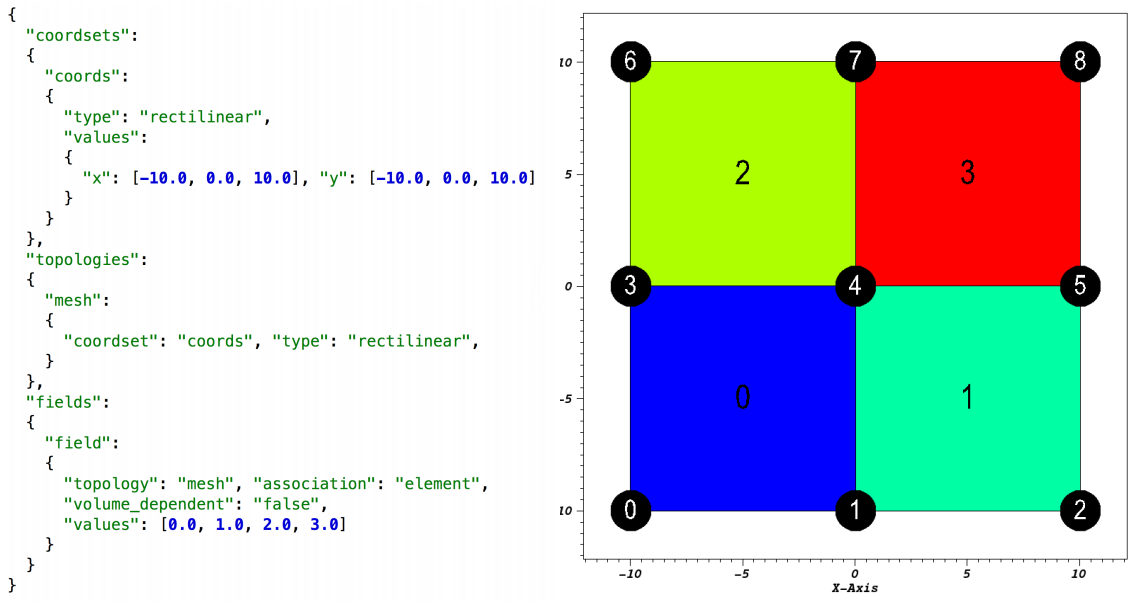
\includegraphics[width=0.6\textwidth]{images/conduit_data_example}
\caption{\label{img:conduit_data_example} Json file representing a simple rectilinear mesh and field.}
\end{figure}

%
The control interface has a simple pipeline-based model for processing
data that is easy to understand, yet also has a more complex graph based
model for processing data when the extra complexity is necessary.
%

\begin{figure}
\centering
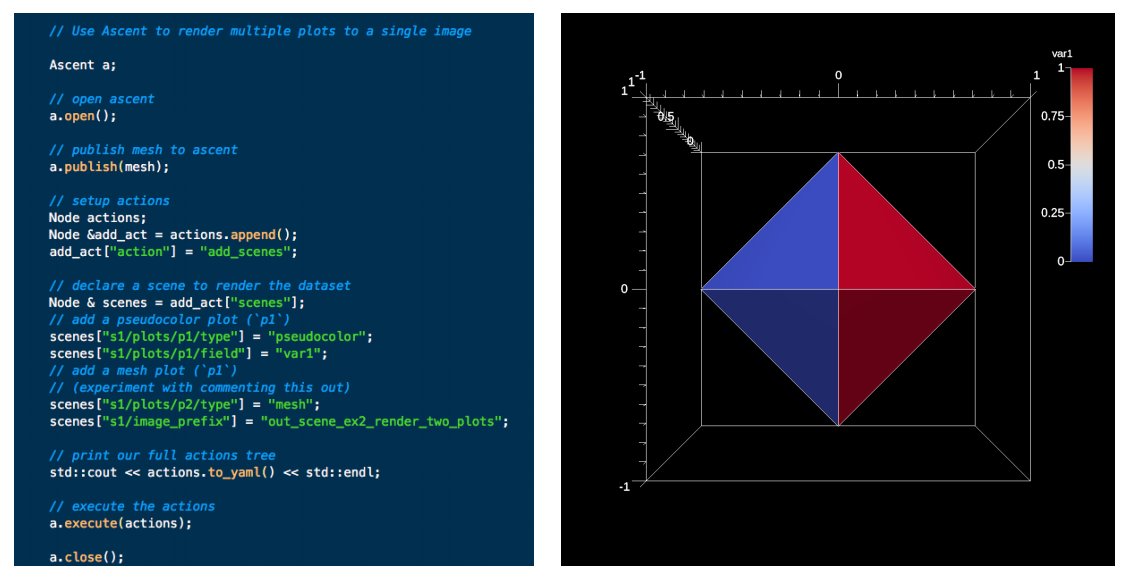
\includegraphics[width=0.6\textwidth]{images/conduit_control_example}
\caption{\label{img:conduit_control_example} C++ rendering actions example and result.}
\end{figure}

\subsection{Create tools to address in situ resource constraints , e.g., a flexible trigger system that allows users to express what is important}

\subsection{Simplify connection to other ecosystems, e.g., python, custom analysis, and Juptyer Notebooks}
